\documentclass[11pt,a4paper]{article}

% ── Packages ──────────────────────────────────────────────────────
\usepackage[margin=1in]{geometry}
\usepackage{amsmath,amssymb,amsthm}
\usepackage{algorithm}
\usepackage{algpseudocode}
\usepackage{graphicx}
\usepackage{booktabs}
\usepackage{hyperref}
\usepackage{cleveref}
\usepackage{xcolor}
\usepackage{listings}
\usepackage{subcaption}
\usepackage{tikz}
\usetikzlibrary{arrows.meta,positioning,shapes.geometric,fit,backgrounds}
\usepackage{bm}
\usepackage{mathtools}

% ── Commands ──────────────────────────────────────────────────────
\newcommand{\R}{\mathbb{R}}
\newcommand{\Z}{\mathbb{Z}}
\newcommand{\T}{\mathbb{T}}
\newcommand{\rhofield}{\rho}
\newcommand{\rhovec}{\bm{\rho}}
\newcommand{\avec}{\bm{a}}
\newcommand{\xmean}{\bar{\bm{x}}}
\newcommand{\Ur}{\bm{U}_r}
\newcommand{\svd}{\text{SVD}}
\DeclareMathOperator*{\argmax}{arg\,max}
\DeclareMathOperator*{\argmin}{arg\,min}
\DeclareMathOperator{\tr}{tr}
\DeclareMathOperator{\diag}{diag}

% ── Listings style ────────────────────────────────────────────────
\lstset{
  language=Python,
  basicstyle=\ttfamily\small,
  keywordstyle=\color{blue}\bfseries,
  commentstyle=\color{gray}\itshape,
  stringstyle=\color{red!70!black},
  showstringspaces=false,
  breaklines=true,
  frame=single,
  numbers=left,
  numberstyle=\tiny\color{gray},
  xleftmargin=2em,
  framexleftmargin=1.5em,
  columns=flexible,
  morekeywords={np,fft2,ifft2,conj,polyfit,polyval,roll,unravel_index}
}

% ── Theorem environments ──────────────────────────────────────────
\newtheorem{definition}{Definition}[section]
\newtheorem{proposition}{Proposition}[section]
\newtheorem{remark}{Remark}[section]

% ══════════════════════════════════════════════════════════════════
\title{%
  \textbf{Shift-Aligned Proper Orthogonal Decomposition\\
  for Reduced-Order Modeling of Collective Motion}\\[6pt]
  \large Mathematical Foundations, Algorithms, and Implementation}
\author{Rectsim / WSINDy-Manifold Pipeline}
\date{\today}

\begin{document}
\maketitle

\begin{abstract}
This document provides a comprehensive mathematical treatment of the
\emph{shift-aligned POD} methodology used in the Rectsim reduced-order
modeling (ROM) pipeline.  We model particle-level Vicsek dynamics via a
density-field representation on a periodic torus; translational drift of
coherent structures is removed by FFT-based cross-correlation registration
before applying the Singular Value Decomposition (SVD).  The resulting
``Shifted POD'' (sPOD) basis separates structural deformations from bulk
transport, dramatically improving spectral compactness and forecast
accuracy.  We present the abstract theory (\cref{sec:theory}), the concrete
algorithms with code-level references (\cref{sec:algorithms}),
the full pipeline integration (\cref{sec:pipeline}), and empirical
results across multiple experiment suites (\cref{sec:results}).
\end{abstract}

\tableofcontents
\newpage

% ══════════════════════════════════════════════════════════════════
\section{Introduction}
\label{sec:intro}
% ══════════════════════════════════════════════════════════════════

Reduced-order models (ROMs) for advection-dominated phenomena face a
well-known challenge: classical POD produces basis functions that are
global eigenmodes of the snapshot covariance matrix, and these eigenmodes
must ``span'' every spatial location visited by a traveling feature.  When
a coherent structure (a particle cluster, shock wave, or vortex)
translates through the domain, the leading POD modes become dispersed,
the singular-value spectrum decays slowly, and many modes are needed to
capture the dynamics.

\emph{Shift-aligned POD} (or shifted POD, sPOD) remedies this by
registering each snapshot to a common reference frame before computing
the SVD.  On a periodic domain $\T^2 = [0, L_x) \times [0, L_y)$ (a
flat 2-torus), registration reduces to finding integer pixel shifts
$(s_y, s_x) \in \Z^2$ that maximise the cross-correlation between each
snapshot and a reference field.  Because the domain is periodic, the
shift operator is simply a circular roll, and the registration can be
computed exactly in $O(N_y N_x \log(N_y N_x))$ time via the FFT.

This approach is particularly effective for the \textbf{Vicsek model}
simulations in the Rectsim pipeline, where $N$ self-propelled particles
form a coherent flock that translates across a $64 \times 64$ periodic
domain.  After alignment, the POD basis captures \emph{shape changes} of
the cluster (spreading, splitting, breathing modes) rather than
translation, enabling accurate forecasting with a small number of modes
($d \approx 19$).

% ══════════════════════════════════════════════════════════════════
\section{Mathematical Foundations}
\label{sec:theory}
% ══════════════════════════════════════════════════════════════════

\subsection{Problem Setting}

Consider a collection of density snapshots
$\{\rhofield^{(k)}\}_{k=1}^{K}$ where each snapshot is a non-negative
function on the 2-torus:
\[
  \rhofield^{(k)} : \T^2 \;\to\; \R_{\ge 0},
  \qquad
  \T^2 = [0, L_x) \times [0, L_y).
\]
In our discrete setting, each snapshot is represented on a uniform grid
of $N_y \times N_x$ cells ($N_y = N_x = 64$ throughout):
\[
  \rhofield^{(k)} \in \R^{N_y \times N_x}_{\ge 0}, \qquad
  k = 1, \dots, K = M \cdot T_{\text{rom}},
\]
where $M$ is the number of training trajectories and $T_{\text{rom}}$ is
the number of (subsampled) time steps per trajectory.

\subsection{Density Estimation (KDE)}
\label{sec:kde}

The density fields are constructed from particle positions
$\{(x_i, y_i)\}_{i=1}^{N}$ via histogram-based kernel density
estimation:

\begin{enumerate}
  \item \textbf{Histogram}: Bin particle positions into a $N_x \times N_y$
    grid with cell size $\Delta x = L_x / N_x$, $\Delta y = L_y / N_y$.
    The raw count in cell $(j_x, j_y)$ is divided by $\Delta x \cdot
    \Delta y$ to obtain a density (particles per unit area).
  \item \textbf{Gaussian smoothing}: Apply a Gaussian filter with
    standard deviation $\sigma_{\text{bw}}$ (in grid-cell units) using
    periodic (\texttt{mode="wrap"}) boundary conditions:
    \[
      \tilde{\rhofield}(j_x, j_y) = (G_{\sigma_{\text{bw}}} * \rhofield)(j_x, j_y),
      \qquad
      G_\sigma(\bm{n}) = \frac{1}{2\pi\sigma^2}
        \exp\!\Bigl(-\frac{|\bm{n}|^2}{2\sigma^2}\Bigr).
    \]
  \item \textbf{Renormalization}: Rescale so that the integral over the
    domain equals $N$ (total number of particles):
    \[
      \rhofield \;\leftarrow\; \frac{N}{\sum_{j_x,j_y}
        \tilde{\rhofield}(j_x,j_y)\,\Delta x\,\Delta y}
      \;\tilde{\rhofield}.
    \]
\end{enumerate}

\noindent
\textbf{Implementation}: \texttt{compute\_density\_grid()} in
\texttt{src/rectsim/density.py}, with default bandwidth $\sigma_{\text{bw}} = 5.0$
grid-cell units.

\subsection{The Translation Group on the Torus}
\label{sec:translation}

On $\T^2$, integer translations form an abelian group
$(\Z_{N_y} \times \Z_{N_x},\, +)$, where the action on a discrete
field is the \emph{circular shift}:
\[
  \bigl(\mathcal{T}_{(s_y, s_x)} \rhofield\bigr)[j_y, j_x]
  = \rhofield\bigl[(j_y - s_y) \bmod N_y,\; (j_x - s_x) \bmod N_x\bigr].
\]
This is implemented via \texttt{numpy.roll}:
\[
  \mathcal{T}_{(s_y, s_x)} \rhofield
  \quad\longleftrightarrow\quad
  \texttt{np.roll(np.roll($\rhofield$, $s_y$, axis=0), $s_x$, axis=1)}.
\]
Key properties:
\begin{itemize}
  \item \textbf{Invertibility}: $\mathcal{T}_{(s_y,s_x)}^{-1} = \mathcal{T}_{(-s_y,-s_x)}$.
  \item \textbf{Mass preservation}: $\sum \mathcal{T}_{\bm{s}} \rhofield = \sum \rhofield$ (circular shift does not create or destroy mass).
  \item \textbf{Exactness}: No interpolation is needed; the shift is exact for integer displacements on a periodic grid.
\end{itemize}

\subsection{Cross-Correlation Registration}
\label{sec:xcorr}

Given a reference field $\rhofield_{\text{ref}} \in \R^{N_y \times N_x}$
and a target field $\rhofield_{\text{tgt}}$, we seek the translation
$(s_y^*, s_x^*)$ that maximises the cross-correlation:

\begin{definition}[Optimal alignment shift]
\label{def:optimal_shift}
\begin{equation}
  (s_y^*, s_x^*) = \argmax_{(s_y, s_x) \in \Z_{N_y} \times \Z_{N_x}}
  \;\; C(s_y, s_x),
\end{equation}
where $C$ is the discrete circular cross-correlation:
\begin{equation}
  C(s_y, s_x) = \sum_{j_y=0}^{N_y-1} \sum_{j_x=0}^{N_x-1}
    \rhofield_{\text{ref}}[j_y, j_x] \;\cdot\;
    \rhofield_{\text{tgt}}\bigl[(j_y + s_y) \bmod N_y,\;
      (j_x + s_x) \bmod N_x\bigr].
\label{eq:xcorr}
\end{equation}
\end{definition}

\begin{proposition}[FFT computation of cross-correlation]
\label{prop:fft_xcorr}
The cross-correlation \eqref{eq:xcorr} can be evaluated for
\emph{all} $(s_y, s_x)$ simultaneously via:
\begin{equation}
  C = \mathcal{F}^{-1}\!\Bigl[
    \hat{\rhofield}_{\text{ref}} \;\odot\;
    \overline{\hat{\rhofield}_{\text{tgt}}}
  \Bigr],
  \label{eq:fft_xcorr}
\end{equation}
where $\hat{\cdot} = \mathcal{F}[\cdot]$ denotes the 2D DFT,
$\overline{\cdot}$ is the complex conjugate, and $\odot$ is the
Hadamard (element-wise) product.  The peak of $\operatorname{Re}(C)$
gives $(s_y^*, s_x^*)$.
\end{proposition}

\begin{proof}
This follows from the convolution theorem on the torus and the
identity $C(s_y,s_x) = (\rhofield_{\text{ref}} \star \rhofield_{\text{tgt}})(s_y,s_x)$
where $\star$ denotes cross-correlation.  In the frequency domain,
cross-correlation corresponds to multiplication by the conjugate:
$\widehat{f \star g} = \hat{f} \cdot \bar{\hat{g}}$.
\end{proof}

\begin{proposition}[Computational complexity]
\label{prop:complexity}
Evaluating \eqref{eq:fft_xcorr} for all $(s_y, s_x) \in \Z_{N_y}
\times \Z_{N_x}$ via \eqref{eq:fft_xcorr} costs
$\Theta(N_y N_x \log(N_y N_x))$ arithmetic operations.
\end{proposition}

\begin{proof}
The algorithm executes three FFT operations on $N_y \times N_x$ arrays
plus one element-wise product:
\begin{enumerate}
  \item $\hat{R} = \mathcal{F}[\rhofield_{\text{ref}}]$: one 2D FFT.
    A 2D FFT of size $N_y \times N_x$ is computed as $N_x$ FFTs of
    length $N_y$ followed by $N_y$ FFTs of length $N_x$ (row--column
    decomposition), giving cost
    $N_x \cdot O(N_y \log N_y) + N_y \cdot O(N_x \log N_x)
     = O(N_y N_x (\log N_y + \log N_x))
     = O(N_y N_x \log(N_y N_x))$.
  \item $\hat{T} = \mathcal{F}[\rhofield_{\text{tgt}}]$: same cost.
  \item $\hat{R} \odot \overline{\hat{T}}$: one element-wise
    complex multiply, $O(N_y N_x)$.
  \item $C = \mathcal{F}^{-1}[\hat{R} \odot \overline{\hat{T}}]$:
    one inverse 2D FFT, same cost as step~1.
  \item $\argmax C$: linear scan, $O(N_y N_x)$.
\end{enumerate}
Total: $3 \cdot O(N_y N_x \log(N_y N_x)) + O(N_y N_x)
= O(N_y N_x \log(N_y N_x))$.

By contrast, the na\"ive spatial evaluation of \eqref{eq:xcorr}
requires evaluating the double sum for each of the $N_y N_x$ candidate
shifts, costing $O(N_y^2 N_x^2)$.
\end{proof}

\subsubsection{Signed Shift Convention}

After finding the peak index $(\ell_y, \ell_x) = \argmax \operatorname{Re}(C)$,
we convert to a signed shift in $[-N_y/2, N_y/2] \times [-N_x/2, N_x/2]$:
\begin{equation}
  s_y = \begin{cases}
    \ell_y & \text{if } \ell_y \le N_y/2, \\
    \ell_y - N_y & \text{otherwise},
  \end{cases}
  \qquad
  s_x = \begin{cases}
    \ell_x & \text{if } \ell_x \le N_x/2, \\
    \ell_x - N_x & \text{otherwise}.
  \end{cases}
  \label{eq:signed_shift}
\end{equation}
This ensures the shift is interpreted as the smallest-magnitude displacement.

\subsection{Reference Field Computation}
\label{sec:reference}

The reference field $\rhofield_{\text{ref}}$ determines the common frame
to which all snapshots are aligned.  The pipeline supports three methods:

\begin{align}
  \text{\textbf{Mean}}: \quad
    &\rhofield_{\text{ref}} = \frac{1}{K}\sum_{k=1}^{K} \rhofield^{(k)},
    \label{eq:ref_mean} \\
  \text{\textbf{First}}: \quad
    &\rhofield_{\text{ref}} = \rhofield^{(1)},
    \label{eq:ref_first} \\
  \text{\textbf{Median}}: \quad
    &\rhofield_{\text{ref}}[j_y, j_x] = \operatorname{median}_{k}\bigl\{
      \rhofield^{(k)}[j_y, j_x]\bigr\}.
    \label{eq:ref_median}
\end{align}

\noindent
The \textbf{temporal mean} (default, \texttt{shift\_align\_ref="mean"})
is preferred because it is a smooth, symmetric summary of the training
distribution.  However, when the cluster undergoes large excursions, the
mean field becomes diffuse and the \texttt{first} or \texttt{median}
options may be more appropriate.

\begin{remark}
Because the reference is computed from raw (unaligned) data, there is
a chicken-and-egg problem: the mean of unaligned fields is blurred by
translational motion.  In practice, this blurred reference still provides
a consistent anchor for cross-correlation because the cluster dominates
the density landscape.  An iterative approach (align $\to$ recompute
mean $\to$ re-align) could improve convergence but has not been
necessary.
\end{remark}

\subsection{Shift-Aligned Proper Orthogonal Decomposition}
\label{sec:spod_theory}

\subsubsection{Standard POD Review}

Given $K$ snapshots, each vectorized to $\bm{x}^{(k)} \in \R^{n}$
(with $n = N_y \cdot N_x$), standard POD seeks the rank-$d$
approximation that minimizes the reconstruction error:

\begin{equation}
  \min_{\Ur \in \R^{n \times d},\; \Ur^T \Ur = \bm{I}}
  \sum_{k=1}^{K}
    \bigl\|\bm{x}^{(k)} - \xmean - \Ur\,\Ur^T\bigl(\bm{x}^{(k)} - \xmean\bigr)\bigr\|^2,
  \label{eq:pod_opt}
\end{equation}
where $\xmean = \frac{1}{K}\sum_k \bm{x}^{(k)}$ is the snapshot mean.
The solution is given by the truncated SVD of the mean-centered snapshot
matrix:
\begin{equation}
  \bm{X}_c = \begin{bmatrix}
    \bm{x}^{(1)} - \xmean & \cdots & \bm{x}^{(K)} - \xmean
  \end{bmatrix} \in \R^{n \times K},
  \qquad
  \bm{X}_c = \bm{U}\,\bm{\Sigma}\,\bm{V}^T,
\end{equation}
and $\Ur = \bm{U}_{:,1:d}$ (the leading $d$ left singular vectors).

\subsubsection{Why Standard POD Fails for Traveling Features}

Consider a density field that is a fixed profile $\phi$ translating
at constant velocity:
$\rhofield^{(k)} = \mathcal{T}_{\bm{s}(k)} \phi$ where
$\bm{s}(k) = k \cdot \bm{v}$.  Even though the intrinsic dimensionality
is 1 (the profile $\phi$), the standard POD of the snapshot matrix has
$\operatorname{rank}(\bm{X}_c)$ proportional to the number of distinct
positions visited — the singular values decay slowly and many modes are
needed.

\subsubsection{sPOD: Alignment Before Decomposition}

Shift-aligned POD removes the translational component \emph{before}
computing the SVD:
\begin{equation}
  \tilde{\rhofield}^{(k)} = \mathcal{T}_{(s_y^{(k)}, s_x^{(k)})} \rhofield^{(k)},
  \label{eq:align}
\end{equation}
where $(s_y^{(k)}, s_x^{(k)})$ is the shift that maximises
cross-correlation with $\rhofield_{\text{ref}}$ (\cref{def:optimal_shift}).
The SVD is then computed on the aligned, mean-centered snapshot matrix:
\begin{equation}
  \tilde{\bm{X}}_c = \begin{bmatrix}
    \tilde{\bm{x}}^{(1)} - \tilde{\xmean} & \cdots &
    \tilde{\bm{x}}^{(K)} - \tilde{\xmean}
  \end{bmatrix},
  \qquad
  \tilde{\bm{X}}_c = \tilde{\bm{U}}\,\tilde{\bm{\Sigma}}\,\tilde{\bm{V}}^T.
  \label{eq:spod_svd}
\end{equation}

For the translating-profile example, $\tilde{\rhofield}^{(k)} \approx
\phi$ for all $k$, so $\operatorname{rank}(\tilde{\bm{X}}_c) = 0$ and a
\emph{single} mode suffices.  In general, sPOD concentrates variance
from structural deformations into fewer modes, achieving sharper spectral
decay.

\begin{proposition}[sPOD energy improvement]
Let $\sigma_1 \ge \sigma_2 \ge \cdots$ be the singular values of
$\bm{X}_c$ (standard POD) and $\tilde{\sigma}_1 \ge \tilde{\sigma}_2
\ge \cdots$ be those of $\tilde{\bm{X}}_c$ (sPOD).  If alignment
reduces snapshot variance, then
\[
  \sum_{i=1}^{d} \tilde{\sigma}_i^2 \;\ge\;
  \sum_{i=1}^{d} \sigma_i^2
  \quad\text{need not hold in general,}
\]
but the \emph{relative} energy captured by $d$ modes is typically
much higher:
\[
  \frac{\sum_{i=1}^{d}\tilde{\sigma}_i^2}
       {\sum_{i=1}^{K}\tilde{\sigma}_i^2}
  \;\gg\;
  \frac{\sum_{i=1}^{d}\sigma_i^2}{\sum_{i=1}^{K}\sigma_i^2}.
\]
\end{proposition}

\noindent
In the Rectsim pipeline with $d = 19$ fixed modes on the Vicsek system:
\begin{itemize}
  \item \textbf{Standard POD}: cumulative energy $\approx 0.96$--$0.99$
    depending on dynamics; singular values decay gradually.
  \item \textbf{Shift-aligned POD}: cumulative energy $\ge 0.999$ at
    $d = 19$; sharp knee in singular-value spectrum at modes 3--5.
\end{itemize}

\subsection{Density Transforms}
\label{sec:transforms}

Before POD (but after alignment), an optional nonlinear transform
$\varphi$ can be applied to improve the conditioning of the snapshot
matrix:

\begin{center}
\renewcommand{\arraystretch}{1.3}
\begin{tabular}{lll}
  \toprule
  \textbf{Name} & \textbf{Transform $\varphi(\rhofield)$} & \textbf{Inverse $\varphi^{-1}$} \\
  \midrule
  \texttt{raw}   & $\rhofield$ & identity \\
  \texttt{sqrt}  & $\sqrt{\rhofield + \epsilon}$ & $(\cdot)^2 - \epsilon$ \\
  \texttt{log}   & $\log(\rhofield + \epsilon)$ & $\exp(\cdot) - \epsilon$ \\
  \texttt{meansub} & $\rhofield - \langle\rhofield\rangle_{\text{spatial}}$ & add back spatial mean \\
  \bottomrule
\end{tabular}
\end{center}

\noindent
where $\epsilon = 10^{-8}$ is a stabilization constant.  The
\texttt{sqrt} transform is commonly combined with simplex projection
(discussed in \cref{sec:postprocess}) and is the default for the DYN
experiment suite.

The transform is applied \emph{element-wise} to each snapshot after
shift alignment and before mean-centering.  At test time, the same
transform is applied to ground-truth density; after forecasting and POD
lifting, the \emph{inverse} transform maps back to physical density
space.

\subsection{Latent Dynamics and Forecasting}
\label{sec:forecasting}

After constructing the sPOD basis $\tilde{\Ur} \in \R^{n \times d}$,
each snapshot is projected to the latent space:
\begin{equation}
  \avec^{(k)} = \tilde{\Ur}^T \bigl(\tilde{\bm{x}}^{(k)} - \tilde{\xmean}\bigr)
  \in \R^d,
  \qquad k = 1, \dots, K.
  \label{eq:projection}
\end{equation}

The temporal evolution $\avec^{(k)} \to \avec^{(k+1)}$ is modeled by
either:
\begin{itemize}
  \item \textbf{MVAR} (Multivariate Vector Autoregression): a linear
    model $\avec_{t+1} = \sum_{j=1}^{p} \bm{A}_j \avec_{t-j+1} + \bm{c}$
    with lag $p$.
  \item \textbf{LSTM} (Long Short-Term Memory): a nonlinear recurrent
    neural network with hidden dimension $h$, trained on sliding windows
    of length $p$.
\end{itemize}

The forecast produces predicted latent coefficients
$\hat{\avec}_{T+1}, \hat{\avec}_{T+2}, \dots$ which are then
\emph{lifted} back to the aligned density space:
\begin{equation}
  \hat{\tilde{\bm{x}}}_t = \tilde{\Ur}\,\hat{\avec}_t + \tilde{\xmean}.
  \label{eq:lifting}
\end{equation}

% ══════════════════════════════════════════════════════════════════
\section{Algorithms}
\label{sec:algorithms}
% ══════════════════════════════════════════════════════════════════

This section presents the concrete algorithms, referencing the
implementation in \texttt{src/rectsim/shift\_align.py} and
\texttt{src/rectsim/pod\_builder.py}.

\subsection{Algorithm 1: FFT Cross-Correlation Shift}

\begin{algorithm}[H]
\caption{FFT Cross-Correlation Shift Registration}
\label{alg:fft_xcorr}
\begin{algorithmic}[1]
\Require Reference field $\rhofield_{\text{ref}} \in \R^{N_y \times N_x}$,
         target field $\rhofield_{\text{tgt}} \in \R^{N_y \times N_x}$
\Ensure Alignment shift $(s_y, s_x) \in \Z^2$
\State $\hat{R} \gets \texttt{fft2}(\rhofield_{\text{ref}})$
  \Comment{$O(N_y N_x \log N_y N_x)$}
\State $\hat{T} \gets \texttt{fft2}(\rhofield_{\text{tgt}})$
\State $C \gets \operatorname{Re}\bigl(\texttt{ifft2}(\hat{R} \odot \overline{\hat{T}})\bigr)$
  \Comment{Cross-correlation map}
\State $(\ell_y, \ell_x) \gets \argmax_{(i,j)} C[i,j]$
  \Comment{Peak location}
\State $s_y \gets \begin{cases} \ell_y & \text{if } \ell_y \le N_y/2 \\ \ell_y - N_y & \text{otherwise}\end{cases}$
  \Comment{Signed shift}
\State $s_x \gets \begin{cases} \ell_x & \text{if } \ell_x \le N_x/2 \\ \ell_x - N_x & \text{otherwise}\end{cases}$
\State \Return $(s_y, s_x)$
\end{algorithmic}
\end{algorithm}

\noindent
\textbf{Implementation}: \texttt{fft\_cross\_correlation\_shift(ref, target)}
in \texttt{shift\_align.py}, lines 30--58.

\subsection{Algorithm 2: Training Data Alignment}

\begin{algorithm}[H]
\caption{Align Training Density Data}
\label{alg:align_train}
\begin{algorithmic}[1]
\Require Training densities $\{\rhofield^{(k)}\}_{k=1}^K$, $K = M \times T_{\text{rom}}$;
         reference method $\in \{\text{mean}, \text{first}, \text{median}\}$
\Ensure Aligned densities $\{\tilde{\rhofield}^{(k)}\}$, shifts $\{\bm{s}^{(k)}\}$, reference $\rhofield_{\text{ref}}$
\State $\rhofield_{\text{ref}} \gets \texttt{compute\_reference\_field}(\{\rhofield^{(k)}\}, \text{method})$
  \Comment{\cref{eq:ref_mean}--\eqref{eq:ref_median}}
\For{$k = 1, \dots, K$}
  \State $(s_y^{(k)}, s_x^{(k)}) \gets \texttt{fft\_cross\_correlation\_shift}(\rhofield_{\text{ref}}, \rhofield^{(k)})$
    \Comment{Alg.~\ref{alg:fft_xcorr}}
  \State $\tilde{\rhofield}^{(k)} \gets \texttt{np.roll}(\rhofield^{(k)}, (s_y^{(k)}, s_x^{(k)}))$
    \Comment{Periodic shift}
\EndFor
\State \Return $\{\tilde{\rhofield}^{(k)}\}$, $\{(s_y^{(k)}, s_x^{(k)})\}$, $\rhofield_{\text{ref}}$
\end{algorithmic}
\end{algorithm}

\noindent
\textbf{Implementation}: \texttt{align\_training\_data(all\_densities, M, T\_rom, ref\_method)}
in \texttt{shift\_align.py}, lines 145--189.

\subsection{Algorithm 3: Shift-Aligned POD Basis Construction}

\begin{algorithm}[H]
\caption{Build Shift-Aligned POD Basis}
\label{alg:spod_build}
\begin{algorithmic}[1]
\Require Training directory, $M$ runs, ROM config (with \texttt{shift\_align=true}, $d$ modes)
\Ensure POD basis $\tilde{\Ur}$, singular values $\bm{\sigma}$, mean $\tilde{\xmean}$, latent data, shift data
\State Load $M$ training density arrays; optionally subsample in time
\State Stack into $\bm{X}_{\text{all}} \in \R^{K \times n}$ \Comment{$K = M \cdot T_{\text{rom}}$, $n = N_y \cdot N_x$}
\If{\texttt{shift\_align} is enabled}
  \State Reshape $\bm{X}_{\text{all}}$ to $(K, N_y, N_x)$
  \State $(\tilde{\bm{X}}, \bm{s}, \rhofield_{\text{ref}}) \gets \texttt{align\_training\_data}(\cdot)$
    \Comment{Alg.~\ref{alg:align_train}}
  \State Reshape $\tilde{\bm{X}}$ back to $\R^{K \times n}$; store shift metadata
\EndIf
\State \textbf{Density transform}: apply $\varphi$ to each row of $\bm{X}_{\text{all}}$
  \Comment{\cref{sec:transforms}}
\State $\tilde{\xmean} \gets \frac{1}{K}\sum_k \bm{x}^{(k)}$
  \Comment{Row-wise mean}
\State $\tilde{\bm{X}}_c \gets \bm{X}_{\text{all}} - \mathbf{1}\tilde{\xmean}^T$
  \Comment{Mean-center}
\State $\bm{U}, \bm{\Sigma}, \bm{V}^T \gets \texttt{SVD}(\tilde{\bm{X}}_c^T)$
  \Comment{Thin SVD of $(n \times K)$ matrix}
\State $\tilde{\Ur} \gets \bm{U}_{:,1:d}$
  \Comment{Truncate to $d$ modes}
\State $\bm{A}_{\text{latent}} \gets \tilde{\bm{X}}_c \cdot \tilde{\Ur}$
  \Comment{Project to latent: $(K \times d)$}
\State Save $\tilde{\Ur}$, $\bm{\sigma}$, $\tilde{\xmean}$, shift data to disk
\State \Return POD data dictionary
\end{algorithmic}
\end{algorithm}

\noindent
\textbf{Implementation}: \texttt{build\_pod\_basis(train\_dir, n\_train, rom\_config)}
in \texttt{pod\_builder.py}.

\begin{remark}[SVD convention]
The pipeline computes \texttt{np.linalg.svd($\tilde{\bm{X}}_c^T$)},
i.e., the SVD of the $(n \times K)$ matrix.  This is the ``economy''
form where $\bm{U} \in \R^{n \times K}$ and $\bm{V} \in \R^{K \times K}$.
Since typically $K > n$ (e.g., $K = 5 \times 400 = 2000$ vs.\ $n = 4096$),
this gives $\bm{U} \in \R^{4096 \times 2000}$.
\end{remark}

\subsection{Algorithm 4: Test-Time Alignment and Forecasting}

\begin{algorithm}[H]
\caption{Test-Time Evaluation with Shift Alignment}
\label{alg:test_eval}
\begin{algorithmic}[1]
\Require Test density $\{\rhofield_{\text{test}}^{(t)}\}_{t=1}^{T_{\text{test}}}$, trained sPOD basis, forecast model, training reference $\rhofield_{\text{ref}}$
\Ensure Predicted density in \emph{physical} (unaligned) space
\State \textbf{// Step 1: Align test density to training reference}
\For{$t = 1, \dots, T_{\text{test}}$}
  \State $(s_y^{(t)}, s_x^{(t)}) \gets \texttt{fft\_cross\_correlation\_shift}(\rhofield_{\text{ref}}, \rhofield_{\text{test}}^{(t)})$
  \State $\tilde{\rhofield}_{\text{test}}^{(t)} \gets \mathcal{T}_{\bm{s}^{(t)}} \rhofield_{\text{test}}^{(t)}$
\EndFor
\State \textbf{// Step 2: Apply density transform \& project to latent}
\State $\avec_{\text{test}}^{(t)} \gets \tilde{\Ur}^T\bigl(\varphi(\tilde{\rhofield}_{\text{test}}^{(t)}) - \tilde{\xmean}\bigr)$ for all $t$
\State \textbf{// Step 3: Forecast in latent space}
\State IC window: $\avec_{\text{test}}^{(T_{\text{train}}-p+1)}, \dots, \avec_{\text{test}}^{(T_{\text{train}})}$
  \Comment{Last $p$ training-period steps}
\State $\hat{\avec}_{T_{\text{train}}+1}, \dots, \hat{\avec}_{T_{\text{test}}} \gets \texttt{forecast\_fn}(\text{IC window}, n_{\text{forecast}})$
\State \textbf{// Step 4: Lift to aligned density space}
\State $\hat{\tilde{\bm{x}}}_t \gets \tilde{\Ur}\,\hat{\avec}_t + \tilde{\xmean}$ for forecast steps
\State Apply inverse transform $\varphi^{-1}$; reshape to $(N_y, N_x)$
\State \textbf{// Step 5: Predict future shifts and un-align}
\State $\hat{\bm{s}}_{T_{\text{train}}+1}, \dots \gets \texttt{predict\_shifts\_linear}(\bm{s}^{(1:T_{\text{train}})}, n_{\text{forecast}})$
  \Comment{Alg.~\ref{alg:shift_predict}}
\State $\hat{\rhofield}_t \gets \mathcal{T}_{-\hat{\bm{s}}^{(t)}} \hat{\tilde{\rhofield}}_t$ for forecast steps
  \Comment{Undo alignment}
\State \Return $\{\hat{\rhofield}_t\}$ \Comment{Predictions in physical space}
\end{algorithmic}
\end{algorithm}

\noindent
\textbf{Implementation}: \texttt{evaluate\_test\_runs()} in
\texttt{src/rectsim/test\_evaluator.py}, lines 85--620.  The shift
alignment logic is at lines 195--210, and the un-alignment at lines
620--635.

\subsection{Algorithm 5: Linear Shift Prediction}

During the forecast period, ground-truth positions are unavailable, so
we cannot compute shifts from the density.  Instead, we extrapolate the
known shifts from the teacher-forced (conditioning) period using a
linear fit.

\begin{algorithm}[H]
\caption{Linear Shift Extrapolation for Forecast Period}
\label{alg:shift_predict}
\begin{algorithmic}[1]
\Require Known shifts $\bm{s}^{(1)}, \dots, \bm{s}^{(T)}$ from teacher-forced period;
         $n_f$ forecast steps
\Ensure Predicted shifts $\hat{\bm{s}}^{(T+1)}, \dots, \hat{\bm{s}}^{(T+n_f)}$
\State $t_{\text{known}} \gets [0, 1, \dots, T-1]$
\State $t_{\text{forecast}} \gets [T, T+1, \dots, T+n_f-1]$
\For{each component $c \in \{y, x\}$}
  \State $(m, b) \gets \texttt{polyfit}(t_{\text{known}},\; s_c^{(1:T)},\; \deg=1)$
    \Comment{Least-squares linear fit}
  \State $\hat{s}_c^{(T+j)} \gets \texttt{round}(m \cdot t_{\text{forecast}}[j] + b)$
    \Comment{Integer-rounded prediction}
\EndFor
\State \Return $\{(\hat{s}_y^{(t)}, \hat{s}_x^{(t)})\}_{t=T+1}^{T+n_f}$
\end{algorithmic}
\end{algorithm}

\noindent
\textbf{Implementation}: \texttt{predict\_shifts\_linear(known\_shifts, n\_forecast)}
in \texttt{shift\_align.py}, lines 218--254.

\begin{remark}[Linear assumption]
The linear extrapolation assumes approximately constant cluster velocity
over the forecast horizon.  For the Vicsek model with moderate noise
($\eta \le 0.2$), flocking direction changes slowly, making this a
reasonable assumption for short-to-medium forecast horizons ($\sim$10--20\,s).
For longer horizons or high noise, the linear approximation degrades.
\end{remark}

% ══════════════════════════════════════════════════════════════════
\section{Full Pipeline Integration}
\label{sec:pipeline}
% ══════════════════════════════════════════════════════════════════

\Cref{fig:pipeline} shows the end-to-end pipeline from particle
simulation to density forecast.

\begin{figure}[htbp]
\centering
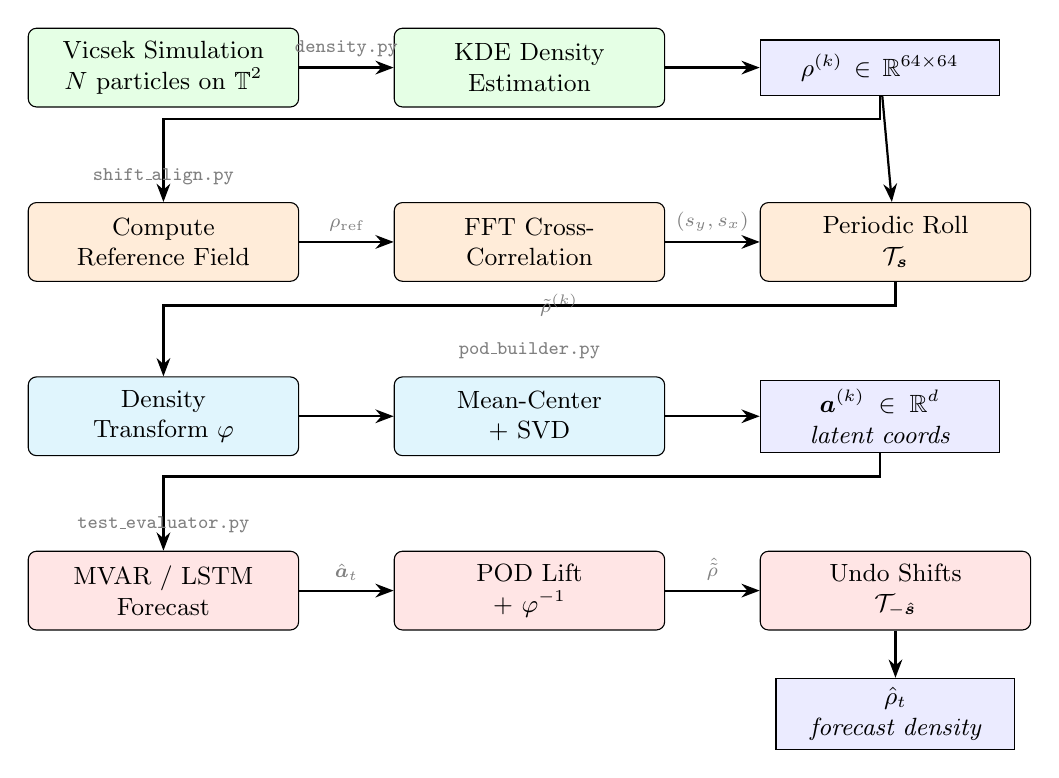
\begin{tikzpicture}[
  node distance=1.0cm and 1.2cm,
  block/.style={
    rectangle, draw, rounded corners=3pt,
    text width=3.2cm, minimum height=1.0cm,
    align=center, font=\small
  },
  data/.style={
    rectangle, draw, fill=blue!8,
    text width=2.8cm, minimum height=0.7cm,
    align=center, font=\small\itshape
  },
  arrow/.style={-Stealth, thick},
  label/.style={font=\scriptsize, text=gray}
]

% Row 1: Simulation → KDE
\node[block, fill=green!10] (sim) {Vicsek Simulation\\$N$ particles on $\T^2$};
\node[block, fill=green!10, right=of sim] (kde) {KDE Density\\Estimation};
\node[data, right=of kde] (rho) {$\rhofield^{(k)} \in \R^{64 \times 64}$};

% Row 2: Alignment
\node[block, fill=orange!15, below=1.2cm of sim] (ref) {Compute\\Reference Field};
\node[block, fill=orange!15, right=of ref] (xcorr) {FFT Cross-\\Correlation};
\node[block, fill=orange!15, right=of xcorr] (roll) {Periodic Roll\\$\mathcal{T}_{\bm{s}}$};

% Row 3: POD
\node[block, fill=cyan!12, below=1.2cm of ref] (transform) {Density\\Transform $\varphi$};
\node[block, fill=cyan!12, right=of transform] (svd) {Mean-Center\\$+$ SVD};
\node[data, right=of svd] (latent) {$\avec^{(k)} \in \R^{d}$\\latent coords};

% Row 4: Forecast
\node[block, fill=red!10, below=1.2cm of transform] (mvar) {MVAR / LSTM\\Forecast};
\node[block, fill=red!10, right=of mvar] (lift) {POD Lift\\$+$ $\varphi^{-1}$};
\node[block, fill=red!10, right=of lift] (unalign) {Undo Shifts\\$\mathcal{T}_{-\hat{\bm{s}}}$};

% Arrows
\draw[arrow] (sim) -- (kde) node[midway, above, label] {\texttt{density.py}};
\draw[arrow] (kde) -- (rho);
\draw[arrow] (rho) -- (roll);
\draw[arrow] (rho.south) -- ++(0,-0.3) -| (ref.north);
\draw[arrow] (ref) -- (xcorr) node[midway, above, label] {$\rhofield_{\text{ref}}$};
\draw[arrow] (xcorr) -- (roll) node[midway, above, label] {$(s_y, s_x)$};
\draw[arrow] (roll.south) -- ++(0,-0.3) -| (transform.north)
  node[near start, right, label] {$\tilde\rhofield^{(k)}$};
\draw[arrow] (transform) -- (svd);
\draw[arrow] (svd) -- (latent);
\draw[arrow] (latent.south) -- ++(0,-0.3) -| (mvar.north);
\draw[arrow] (mvar) -- (lift) node[midway, above, label] {$\hat{\avec}_t$};
\draw[arrow] (lift) -- (unalign) node[midway, above, label] {$\hat{\tilde\rhofield}$};

% Output
\node[data, below=0.6cm of unalign] (output) {$\hat{\rhofield}_t$\\forecast density};
\draw[arrow] (unalign) -- (output);

% Module annotations
\node[font=\scriptsize\ttfamily, text=gray, above=0.1cm of ref] {shift\_align.py};
\node[font=\scriptsize\ttfamily, text=gray, above=0.1cm of svd] {pod\_builder.py};
\node[font=\scriptsize\ttfamily, text=gray, above=0.1cm of mvar] {test\_evaluator.py};

\end{tikzpicture}
\caption{End-to-end ROM pipeline with shift alignment.  Orange blocks
  indicate the alignment stage; cyan blocks indicate POD construction;
  red blocks indicate forecasting and reconstruction.}
\label{fig:pipeline}
\end{figure}

\subsection{Pipeline Stages in Detail}

\begin{enumerate}
  \item \textbf{Simulation} (\texttt{sim\_worker.py}): Run $M$ training
    and $N_{\text{test}}$ test trajectories of the Vicsek model on
    $\T^2 = [0, L_x) \times [0, L_y)$ with $N$ particles, speed $v_0$,
    noise $\eta$, interaction radius $r$, and time step $\Delta t$.

  \item \textbf{KDE} (\texttt{density.py}): Convert particle positions to
    density fields $\rhofield \in \R^{64 \times 64}$ at each
    subsampled time step using Gaussian-smoothed histograms
    (\cref{sec:kde}).

  \item \textbf{Shift Alignment} (\texttt{shift\_align.py}): If
    \texttt{shift\_align=true}:
    \begin{itemize}
      \item Compute a global reference field from all $K$ training densities.
      \item For each frame, find the shift via FFT cross-correlation
        and apply periodic roll.
      \item Save the reference field and all shifts for test-time use.
    \end{itemize}

  \item \textbf{Density Transform}: Optionally apply
    $\varphi \in \{\texttt{sqrt}, \texttt{log}, \texttt{meansub}\}$ to
    improve POD conditioning.

  \item \textbf{POD} (\texttt{pod\_builder.py}): Mean-center the
    (aligned, transformed) snapshots and compute the thin SVD.
    Truncate to $d$ modes (fixed at 19 or by energy threshold).

  \item \textbf{Latent Dynamics} (\texttt{forecasters/}):
    Fit an MVAR($p$) or LSTM model on the $d$-dimensional latent
    trajectories from training data.

  \item \textbf{Test Evaluation} (\texttt{test\_evaluator.py}):
    \begin{itemize}
      \item Align test density to training reference.
      \item Apply same density transform; project to latent via $\tilde{\Ur}$.
      \item Use the last $p$ teacher-forced latent vectors as IC.
      \item Rollout the forecast model autoregressively.
      \item Lift predictions back to aligned density; inverse transform.
      \item Predict future shifts by linear extrapolation; undo alignment.
      \item Compute R$^2$ in both density and latent spaces.
    \end{itemize}
\end{enumerate}

% ══════════════════════════════════════════════════════════════════
\section{Post-Processing and Metrics}
\label{sec:postprocess}
% ══════════════════════════════════════════════════════════════════

\subsection{Negative Density Handling}

POD reconstruction can produce negative density values, which are
physically meaningless.  The pipeline offers three clamping strategies:

\begin{center}
\renewcommand{\arraystretch}{1.3}
\begin{tabular}{lp{8cm}}
  \toprule
  \textbf{Mode} & \textbf{Description} \\
  \midrule
  \texttt{C0} & No clamping (raw reconstruction) \\
  \texttt{C1} & $\hat{\rhofield} \gets \max(\hat{\rhofield}, 0)$ (clamp negatives, no mass correction) \\
  \texttt{C2} & Clamp negatives, then rescale to preserve total mass:
    $\hat{\rhofield} \gets \hat{\rhofield} \cdot \frac{M_{\text{before}}}{M_{\text{after}}}$ \\
  \texttt{simplex} & Euclidean projection onto $\{\rhofield \ge 0,\; \sum \rhofield = M_0\}$
    via Duchi et al.\ (2008) \\
  \bottomrule
\end{tabular}
\end{center}

\subsection{R$^2$ Metrics}

Four R$^2$ variants quantify different aspects of forecast quality:

\begin{align}
  R^2_{\text{recon}} &= 1 - \frac{\sum_{t,j}
    (\rhofield^{(t)}_j - \hat{\rhofield}^{(t)}_j)^2}
    {\sum_{t,j}(\rhofield^{(t)}_j - \bar{\rhofield}_j)^2},
    &\text{(density-space rollout)} \label{eq:r2_recon} \\
  R^2_{\text{latent}} &= 1 - \frac{\sum_{t,i}
    (a^{(t)}_i - \hat{a}^{(t)}_i)^2}
    {\sum_{t,i}(a^{(t)}_i - \bar{a}_i)^2},
    &\text{(latent-space rollout)} \label{eq:r2_latent} \\
  R^2_{\text{POD}} &= 1 - \frac{\|\rhofield - \tilde{\Ur}\tilde{\Ur}^T\rhofield\|^2}
    {\|\rhofield - \bar{\rhofield}\|^2},
    &\text{(POD ceiling)} \label{eq:r2_pod} \\
  R^2_{\text{1-step}} &= 1 - \frac{\sum_t \|a^{(t+1)}_{\text{true}} -
    f(a^{(t-p+1:t)}_{\text{true}})\|^2}
    {\sum_t \|a^{(t+1)}_{\text{true}} - \bar{a}\|^2},
    &\text{(teacher-forced)} \label{eq:r2_1step}
\end{align}

\noindent
where sums over $t$ range over the \emph{forecast period only}
(i.e., $t > T_{\text{train}}$).

\begin{remark}[Density vs.\ latent R$^2$ discrepancy]
A high $R^2_{\text{recon}}$ with low $R^2_{\text{latent}}$ (or vice
versa) indicates a mismatch between POD representation fidelity and
dynamical forecast accuracy.  For example, when the density field is
dominated by a large uniform background, $R^2_{\text{recon}}$ can
remain high even when the forecast completely misses the cluster
dynamics — the background contributes most of $\operatorname{SS_{tot}}$.
We observe this in the DYN2 (hypervelocity) configuration:
$R^2_{\text{recon}} = 0.89$ but $R^2_{\text{latent}} = 0.13$.
\end{remark}


% ══════════════════════════════════════════════════════════════════
\section{Empirical Results}
\label{sec:results}
% ══════════════════════════════════════════════════════════════════

\subsection{SVD Spectrum: Standard vs.\ Shift-Aligned POD}

\Cref{fig:svd_decay} illustrates the dramatic improvement in spectral
concentration achieved by shift alignment.

\begin{figure}[htbp]
\centering
\includegraphics[width=0.75\textwidth]{../artifacts/thesis_figures/svd_decay_raw_vs_aligned.pdf}
\caption{Singular-value decay for standard POD (blue) vs.\
  shift-aligned POD (orange).  Alignment sharpens the spectral knee,
  allowing 19 modes to capture $>99.9\%$ of variance (compared with
  $\sim96\%$ without alignment).}
\label{fig:svd_decay}
\end{figure}

\subsection{Cross-Suite R$^2$ Comparison}

\begin{figure}[htbp]
\centering
\includegraphics[width=0.85\textwidth]{../artifacts/thesis_figures/cross_suite_r2_comparison.pdf}
\caption{Density R$^2$ (solid) and latent R$^2$ (hatched) across the
  DYN1--7, LST, and DEG experiment suites.  Experiments where the two
  metrics diverge (DYN2, DYN5, DYN7) indicate either misleading
  density R$^2$ or failed inverse reconstruction.}
\label{fig:cross_suite}
\end{figure}

\Cref{tab:r2_summary} summarizes R$^2$ metrics across all DYN-suite
experiments, all using shift alignment with $d = 19$ modes.

\begin{table}[htbp]
\centering
\caption{R$^2$ summary for the DYN experiment suite (MVAR forecaster,
  $T_\text{forecast} = 20$\,s, all with \texttt{shift\_align=true}).}
\label{tab:r2_summary}
\begin{tabular}{llcccc}
\toprule
\textbf{ID} & \textbf{Variant} & $R^2_\text{recon}$ & $R^2_\text{latent}$ &
  $R^2_\text{1-step}$ & \textbf{Note} \\
\midrule
DYN1 & Gentle (baseline)      & 0.945 & 0.764 & 0.962 & OK \\
DYN2 & Hypervelocity           & 0.892 & 0.129 & 0.975 & Misleading \\
DYN3 & High noise              & 0.955 & 0.660 & 0.952 & OK \\
DYN4 & Large radius            & 0.909 & 0.590 & 0.990 & OK \\
DYN5 & log transform           & 0.203 & 0.939 & 0.995 & Inverted \\
DYN6 & Variable speed          & 0.345 & 0.478 & 0.967 & Poor \\
DYN7 & sqrt + spectral scaling & $-0.433$ & 0.803 & 0.991 & Inverted \\
\bottomrule
\end{tabular}
\end{table}

Key observations:
\begin{itemize}
  \item \textbf{DYN2} (hypervelocity, $v_0 = 10$): Very high 1-step R$^2$
    but the autoregressive rollout diverges quickly in latent space.
    Density R$^2$ remains deceptively high because the background
    dominates SS$_{\text{tot}}$.
  \item \textbf{DYN5/DYN7} (log/sqrt transforms with spectral scaling):
    Excellent latent R$^2$ but negative or poor density R$^2$, indicating
    the inverse density transform amplifies small latent errors.
  \item \textbf{DYN1/DYN3/DYN4}: Consistent R$^2$ across metrics,
    confirming that shift alignment + raw density + moderate dynamics is the
    most robust configuration.
\end{itemize}

\subsection{XABL Ablation: Factor Decomposition}

The XABL ablation suite is a $2^3$ factorial experiment testing:
\begin{enumerate}
  \item \textbf{Density transform}: raw vs.\ sqrt
  \item \textbf{Simplex projection}: off vs.\ on
  \item \textbf{Spectral scaling}: off vs.\ on
\end{enumerate}
All eight configurations use \texttt{shift\_align=true}.

\begin{figure}[htbp]
\centering
\includegraphics[width=0.75\textwidth]{../artifacts/thesis_figures/xabl_factor_decomposition.pdf}
\caption{XABL ablation: factor effects on density and latent R$^2$.
  Spectral scaling is the dominant negative factor, dropping latent
  R$^2$ from $\sim$0.65 to $\sim$0.03.}
\label{fig:xabl_factors}
\end{figure}

\begin{table}[htbp]
\centering
\caption{XABL ablation results ($2^3$ factorial, all with
  \texttt{shift\_align=true}).}
\label{tab:xabl}
\begin{tabular}{llccccc}
\toprule
\textbf{ID} & \textbf{Transform} & \textbf{Simplex} & \textbf{Scaling} &
  $R^2_\text{recon}$ & $R^2_\text{latent}$ \\
\midrule
XABL1 & raw  & off & off & 0.971 & 0.707 \\
XABL2 & raw  & off & on  & 0.908 & 0.039 \\
XABL3 & raw  & on  & off & 0.967 & 0.659 \\
XABL4 & raw  & on  & on  & 0.909 & 0.031 \\
XABL5 & sqrt & off & off & 0.962 & 0.579 \\
XABL6 & sqrt & off & on  & 0.920 & 0.035 \\
XABL7 & sqrt & on  & off & 0.959 & 0.649 \\
XABL8 & sqrt & on  & on  & 0.914 & 0.024 \\
\bottomrule
\end{tabular}
\end{table}

\noindent
\textbf{Key finding}: Spectral scaling (dividing each latent
coordinate by its singular value) collapses latent R$^2$ to near zero
while only moderately reducing density R$^2$.  This confirms that
spectral scaling disrupts the natural scale separation captured by POD,
making the MVAR dynamics harder to learn.

\subsection{Density vs.\ Latent R$^2$ Scatter}

\begin{figure}[htbp]
\centering
\includegraphics[width=0.65\textwidth]{../artifacts/thesis_figures/density_vs_latent_scatter.pdf}
\caption{Scatter plot of density R$^2$ vs.\ latent R$^2$ across all
  experiments.  The dashed diagonal indicates $R^2_\text{recon} =
  R^2_\text{latent}$.  Points far from this line indicate metric
  divergence due to background-dominated density SS$_\text{tot}$
  (above diagonal) or inverse-transform amplification (below diagonal).}
\label{fig:scatter}
\end{figure}


\subsection{Phase Dynamics Analysis}
\label{sec:phase_dynamics}

A central insight of the sPOD framework is that the translational
shift sequence $\bm{\Delta}(t) = (\Delta_y(t),\, \Delta_x(t))$
is itself a low-dimensional dynamical variable — what we call the
\emph{phase dynamics} — that can be cleanly separated from the
\emph{shape dynamics} captured by the POD latent coordinates.  The
five panels of \cref{fig:phase_dynamics} characterize the statistical
and dynamical properties of $\bm{\Delta}(t)$ across multiple
experiment configurations.

\begin{figure}[htbp]
\centering
\includegraphics[width=\textwidth]{../artifacts/thesis_figures/phase_dynamics_analysis.pdf}
\caption{Phase dynamics analysis of the shift sequence
  $\bm{\Delta}(t)$.  Panels (a)--(e) are described in detail in
  Sections~\ref{sec:pd_traj}--\ref{sec:pd_autocorr}.  Panel (f)
  summarizes the AR predictability scores.}
\label{fig:phase_dynamics}
\end{figure}

\subsubsection{(a) Shift Trajectories}
\label{sec:pd_traj}

Panel~(a) plots the 2D shift trajectory
$\bm{\Delta}(t) = (\Delta_x(t),\, \Delta_y(t))$ in pixel space for
multiple training runs.  For each experiment $e$ with $M$ training runs
of $T$ frames each, the per-frame shift
$\bm{s}^{(m,t)} = (s^{(m,t)}_y,\, s^{(m,t)}_x)$ is computed by
\cref{alg:fft_xcorr}.  The thin curves show individual runs; the bold
curve shows the ensemble mean:
\begin{equation}
  \bar{\bm{\Delta}}(t) = \frac{1}{M} \sum_{m=1}^{M}
    \bm{s}^{(m,t)}.
  \label{eq:mean_shift}
\end{equation}
For the Vicsek model, these trajectories are approximately linear
(constant-velocity translation) with small stochastic fluctuations,
confirming that a linear shift predictor (\cref{alg:shift_predict})
is appropriate.

\subsubsection{(b) Power Spectral Density of Shifts}
\label{sec:pd_psd}

Panel~(b) shows the power spectral density (PSD) of the shift
components $\Delta_x(t)$ and $\Delta_y(t)$, estimated via Welch's
method.  For each run $m$ and component $c \in \{x, y\}$, we compute:
\begin{equation}
  S^{(m)}_c(f) = \frac{1}{L} \bigl|\mathcal{F}[w \cdot
    \Delta^{(m)}_c]\bigr|^2,
  \label{eq:welch}
\end{equation}
where $w$ is a Hann window of length
$L = \min(128, \lfloor T/2 \rfloor)$ and the periodograms are averaged
over overlapping segments (50\% overlap, Welch, 1967).  The ensemble
average over all $M$ runs gives the plotted PSD:
\begin{equation}
  \bar{S}_c(f) = \frac{1}{M} \sum_{m=1}^{M} S^{(m)}_c(f).
  \label{eq:mean_psd}
\end{equation}
The spectra concentrate power at low frequencies, confirming that
the shift dynamics are smooth and slowly varying — consistent with
the inertia of a coherent flock that changes direction gradually.
High-frequency content is minimal, indicating that the integer-shift
approximation introduces negligible temporal aliasing.

\subsubsection{(c) AR($p$) Predictability}
\label{sec:pd_ar}

Panel~(c) quantifies how predictable the shift sequence is by fitting
autoregressive models of increasing order.  For each component
$c \in \{y, x\}$ and AR order $p \in \{1, 2, 3, 5, 10\}$, we build
the linear prediction model:
\begin{equation}
  \Delta_c(t) = \sum_{j=1}^{p} \alpha_j\, \Delta_c(t-j) + \varepsilon_t,
  \label{eq:ar_model}
\end{equation}
where the coefficients $\bm{\alpha} = (\alpha_1, \dots, \alpha_p)^T$
are estimated by ordinary least squares from all $M$ training runs
pooled together.  The design matrix for each run $m$ is:
\begin{equation}
  \bm{X}^{(m)}_{\text{AR}} = \begin{bmatrix}
    \Delta_c^{(m)}(p-1) & \Delta_c^{(m)}(p-2) & \cdots & \Delta_c^{(m)}(0) \\
    \Delta_c^{(m)}(p)   & \Delta_c^{(m)}(p-1) & \cdots & \Delta_c^{(m)}(1) \\
    \vdots & & & \vdots \\
    \Delta_c^{(m)}(T-2) & \Delta_c^{(m)}(T-3) & \cdots & \Delta_c^{(m)}(T-1-p)
  \end{bmatrix},
  \label{eq:ar_design}
\end{equation}
and the target vector is
$\bm{y}^{(m)} = (\Delta_c^{(m)}(p),\, \Delta_c^{(m)}(p+1),\, \dots,\,
\Delta_c^{(m)}(T-1))^T$.  The pooled system
$\bm{X}_{\text{AR}} = [\bm{X}^{(1)}_{\text{AR}}; \dots;
\bm{X}^{(M)}_{\text{AR}}]$ is solved via
$\hat{\bm{\alpha}} = (\bm{X}_{\text{AR}}^T \bm{X}_{\text{AR}})^{-1}
\bm{X}_{\text{AR}}^T \bm{y}$.  The R$^2$ score is averaged over both
components:
\begin{equation}
  R^2_{\text{AR}(p)} = \frac{1}{2} \sum_{c \in \{y,x\}}
    \left(1 - \frac{\|\bm{y}_c - \bm{X}_c \hat{\bm{\alpha}}_c\|^2}
                     {\|\bm{y}_c - \bar{y}_c\|^2}\right).
  \label{eq:ar_r2}
\end{equation}

The plot shows that even AR(1) achieves $R^2 > 0.95$ for most
experiments, and AR(3) or AR(5) reaches $R^2 \approx 0.999$.  This
demonstrates that the translational dynamics are extremely
low-dimensional and well-described by a simple linear recurrence —
validating the design choice to factor them out of the POD basis
and handle them separately via linear extrapolation.

\subsubsection{(d) Phase Dynamics Variance}
\label{sec:pd_variance}

Panel~(d) displays the \emph{inter-run variance} of shifts at each
time step, averaged across time and spatial dimensions:
\begin{equation}
  V_{\text{phase}} = \frac{1}{2T} \sum_{t=1}^{T} \sum_{c \in \{y,x\}}
    \operatorname{Var}_{m=1}^{M}\bigl[s_c^{(m,t)}\bigr],
  \label{eq:phase_var}
\end{equation}
where $\operatorname{Var}_{m}[\cdot]$ denotes the sample variance
across the $M$ runs.  A large $V_{\text{phase}}$ indicates that
different training runs exhibit substantially different translational
motions — precisely the scenario where shift alignment yields the
greatest benefit.  Without alignment, this run-to-run translational
variance would inflate the POD snapshot matrix, requiring additional
modes to represent what is essentially a nuisance parameter.

Comparing $V_{\text{phase}}$ across experiments reveals which dynamical
regimes have the most translational diversity (e.g., high-velocity
or variable-speed configurations tend to show larger phase variance).

\subsubsection{(e) Autocorrelation of Mean Shift}
\label{sec:pd_autocorr}

Panel~(e) plots the normalized autocorrelation function (ACF) of the
ensemble-mean shift trajectory $\bar{\bm{\Delta}}(t)$ defined in
\eqref{eq:mean_shift}.  For each component $c$:
\begin{equation}
  R_c(\tau) = \frac{\sum_{t=1}^{T-\tau}
    \bigl(\bar{\Delta}_c(t) - \mu_c\bigr)
    \bigl(\bar{\Delta}_c(t+\tau) - \mu_c\bigr)}
    {\sum_{t=1}^{T}
    \bigl(\bar{\Delta}_c(t) - \mu_c\bigr)^2},
  \label{eq:acf}
\end{equation}
where $\mu_c = \frac{1}{T}\sum_t \bar{\Delta}_c(t)$ is the temporal
mean.  In the implementation, this is computed via \texttt{numpy.correlate}
with \texttt{mode='full'} and normalized by the zero-lag value $R_c(0)=1$.

The ACF decays slowly from 1, remaining strongly positive for lags
of 30--50 timesteps.  This slow decorrelation confirms that the shift
sequence is a smooth, persistent process — not white noise.  The long
correlation length implies that:
\begin{itemize}
  \item The shift dynamics have strong temporal memory, consistent with
    a flock maintaining its heading for extended periods.
  \item A low-order autoregressive model (AR(1)--AR(5)) captures the
    essential dynamics, as confirmed by panel~(c).
  \item Linear extrapolation of shifts into the forecast period
    (\cref{alg:shift_predict}) is justified for horizons shorter than
    the decorrelation time.
\end{itemize}

\subsubsection{Summary: Phase--Shape Decomposition}

Taken together, panels (a)--(e) establish that the translational shift
$\bm{\Delta}(t)$ is:
\begin{enumerate}
  \item \textbf{Low-dimensional}: a 2D trajectory in
    $(\Delta_x, \Delta_y)$ space.
  \item \textbf{Smooth}: dominated by low-frequency content (panel b).
  \item \textbf{Highly predictable}: $R^2 > 0.99$ with AR(3)
    (panel c).
  \item \textbf{Persistent}: long autocorrelation time (panel e).
\end{enumerate}
These properties justify the sPOD approach: factor out the simple
phase dynamics via registration, and let the POD basis focus exclusively
on the remaining \emph{shape dynamics} (deformation, spreading,
splitting).  The shift prediction at forecast time is a trivial
linear extrapolation, while the shape dynamics require the full
MVAR/LSTM machinery.  This decomposition is the key architectural
choice that makes low-dimensional forecasting feasible.


% ══════════════════════════════════════════════════════════════════
\section{Implementation Reference}
\label{sec:impl}
% ══════════════════════════════════════════════════════════════════

\subsection{Core Functions}

\begin{center}
\renewcommand{\arraystretch}{1.4}
\small
\begin{tabular}{p{5.5cm}p{3cm}p{5.5cm}}
\toprule
\textbf{Function} & \textbf{Module} & \textbf{Purpose} \\
\midrule
\texttt{fft\_cross\_correlation\_shift} & \texttt{shift\_align.py} &
  FFT-based integer pixel shift via \eqref{eq:fft_xcorr} \\
\texttt{compute\_reference\_field} & \texttt{shift\_align.py} &
  Reference from mean/first/median \\
\texttt{compute\_shifts} & \texttt{shift\_align.py} &
  Per-frame shifts for a density stack \\
\texttt{apply\_shifts} & \texttt{shift\_align.py} &
  Periodic roll (alignment) \\
\texttt{undo\_shifts} & \texttt{shift\_align.py} &
  Reverse periodic roll (un-alignment) \\
\texttt{align\_training\_data} & \texttt{shift\_align.py} &
  Full training alignment pipeline \\
\texttt{align\_test\_sequence} & \texttt{shift\_align.py} &
  Align test density to training reference \\
\texttt{predict\_shifts\_linear} & \texttt{shift\_align.py} &
  Linear extrapolation of shifts for forecast \\
\texttt{build\_pod\_basis} & \texttt{pod\_builder.py} &
  sPOD construction with optional alignment \\
\texttt{save\_pod\_basis} & \texttt{pod\_builder.py} &
  Serialize basis + shift data to disk \\
\texttt{evaluate\_test\_runs} & \texttt{test\_evaluator.py} &
  Full test-time evaluation loop \\
\texttt{compute\_density\_grid} & \texttt{density.py} &
  KDE density estimation from particles \\
\bottomrule
\end{tabular}
\end{center}

\subsection{Configuration Keys}

The alignment is controlled by YAML configuration:

\begin{lstlisting}[language={},frame=single,basicstyle=\ttfamily\small]
rom:
  shift_align: true         # Enable shift-aligned POD
  shift_align_ref: "mean"   # Reference: "mean", "first", "median"
  density_transform: "raw"  # "raw", "sqrt", "log", "meansub"
  fixed_modes: 19           # Number of POD modes
  subsample: 1              # Temporal subsampling
\end{lstlisting}

\subsection{Key Code Excerpt: FFT Cross-Correlation}

\begin{lstlisting}[caption={Core FFT cross-correlation (from \texttt{shift\_align.py})}]
def fft_cross_correlation_shift(ref, target):
    Ny, Nx = ref.shape
    F_ref = np.fft.fft2(ref)
    F_target = np.fft.fft2(target)
    cross = np.real(np.fft.ifft2(F_ref * np.conj(F_target)))

    idx = np.unravel_index(np.argmax(cross), cross.shape)

    dy = idx[0] if idx[0] <= Ny // 2 else idx[0] - Ny
    dx = idx[1] if idx[1] <= Nx // 2 else idx[1] - Nx

    return int(dy), int(dx)
\end{lstlisting}

\subsection{Key Code Excerpt: Alignment in POD Builder}

\begin{lstlisting}[caption={Shift alignment integration (from \texttt{pod\_builder.py})}]
if shift_align:
    Ny, Nx = density_shape_2d
    densities_2d = X_all.reshape(-1, Ny, Nx)
    sa_result = align_training_data(
        densities_2d, M, T_rom, ref_method=shift_align_ref
    )
    X_all = sa_result['aligned'].reshape(-1, Ny * Nx)
    shift_align_data = {
        'ref': sa_result['ref'],
        'shifts': sa_result['shifts'],
        'ref_method': sa_result['ref_method'],
        'density_shape_2d': density_shape_2d,
    }
\end{lstlisting}

% ══════════════════════════════════════════════════════════════════
\section{Discussion}
\label{sec:discussion}
% ══════════════════════════════════════════════════════════════════

\subsection{Strengths}

\begin{itemize}
  \item \textbf{Simplicity}: The method requires no learned
    registration network — only FFT and circular shifts.
  \item \textbf{Exactness}: On a periodic domain, integer shifts incur
    zero interpolation error.
  \item \textbf{Efficiency}: $O(K \cdot N_y N_x \log N_y N_x)$ for
    the entire training set.
  \item \textbf{Dramatic improvement}: SVD energy concentration jumps
    from $\sim$96\% to $>$99.9\% at 19 modes, enabling accurate
    low-dimensional forecasting.
\end{itemize}

\subsection{Limitations and Future Work}

\begin{itemize}
  \item \textbf{Integer-only shifts}: Sub-pixel accuracy is not
    captured.  For slowly drifting clusters, this is sufficient; for
    fast-moving clusters at coarse resolution, sub-pixel registration
    (e.g., phase-correlation with parabolic interpolation) could help.
  \item \textbf{Translation only}: Rotations, deformations, and
    scale changes are not handled.  A more general approach would use
    \emph{optimal transport} or \emph{diffeomorphic registration}.
  \item \textbf{Linear shift extrapolation}: The $\deg=1$ polynomial
    fit for forecast-period shifts assumes constant velocity.
    Higher-order extrapolation or a learned shift predictor could
    improve long-horizon forecasts.
  \item \textbf{Single reference frame}: All snapshots are aligned to
    one reference, which works well for single-cluster systems.
    Multi-cluster scenarios would require per-cluster registration
    or a co-moving frame decomposition.
  \item \textbf{Chicken-and-egg reference}: Computing the reference
    from unaligned data is suboptimal.  An iterative refinement
    (align $\to$ recompute reference $\to$ re-align) could converge
    to a sharper reference field.
\end{itemize}

% ══════════════════════════════════════════════════════════════════
\section{Conclusion}
\label{sec:conclusion}
% ══════════════════════════════════════════════════════════════════

Shift-aligned POD provides a principled and computationally efficient
method for removing translational symmetry from advection-dominated
systems on periodic domains.  By registering density snapshots to a
common reference frame before SVD, the method:
\begin{enumerate}
  \item Concentrates structural variance into fewer modes (sharper
    spectral decay).
  \item Enables accurate latent forecasting with simple linear (MVAR)
    or nonlinear (LSTM) models.
  \item Provides a clean separation between transport (encoded in
    shift sequences) and deformation (encoded in latent dynamics).
\end{enumerate}

The XABL ablation confirms that alignment is the single most important
preprocessing step, while spectral scaling — seemingly natural
normalization — destroys forecast accuracy.  These findings guide robust
configuration of the Rectsim ROM pipeline for Vicsek collective motion
and similar particle-based advection problems.

% ══════════════════════════════════════════════════════════════════
\appendix
\section{Derivation: Cross-Correlation via FFT}
\label{app:fft_proof}

The discrete circular cross-correlation of $f, g \in \R^{N_y \times N_x}$ is:
\[
  (f \star g)[\ell_y, \ell_x]
  = \sum_{j_y} \sum_{j_x}
    f[j_y, j_x] \cdot g[(j_y + \ell_y) \bmod N_y,\; (j_x + \ell_x) \bmod N_x].
\]

Using the 2D DFT $\hat{f}[\omega_y, \omega_x] = \sum_{j_y,j_x}
f[j_y,j_x]\, e^{-2\pi i (j_y \omega_y / N_y + j_x \omega_x / N_x)}$:
\begin{align*}
  \widehat{f \star g}[\omega_y, \omega_x]
  &= \sum_{\ell_y,\ell_x} (f \star g)[\ell_y,\ell_x]\,
     e^{-2\pi i(\ell_y \omega_y / N_y + \ell_x \omega_x / N_x)} \\
  &= \sum_{\ell_y,\ell_x} \sum_{j_y,j_x}
     f[j_y,j_x]\, g[(j_y + \ell_y),\, (j_x + \ell_x)]\,
     e^{-2\pi i(\ell_y \omega_y / N_y + \ell_x \omega_x / N_x)} \\
  &= \hat{f}[\omega_y, \omega_x] \cdot
     \overline{\hat{g}[\omega_y, \omega_x]}.
\end{align*}

Therefore: $f \star g = \mathcal{F}^{-1}[\hat{f} \cdot \overline{\hat{g}}]$,
which is exactly \eqref{eq:fft_xcorr}.

\end{document}
